\documentclass[12pt]{paper}%

\RequirePackage[letterpaper,headsep=0.15in,footskip=0.25in,margin=0.6in,top=0.25in,bottom=0.25in,includeheadfoot]{geometry}
\RequirePackage{fancyhdr}
\RequirePackage{amsmath}

% set the page style
\pagestyle{fancy}
\chead{\fancyplain{}{%
\small \scriptsize{\hspace{-1cm} QC and QA of the NIAK fMRI preprocessing pipeline}
    }
}

\rhead{\begin{footnotesize} Version 1.0  \end{footnotesize}}

\lhead{\fancyplain{}{\begin{footnotesize} SIMEXP \end{footnotesize}}}

% \lfoot{\fancyplain{}{%
%         \ifthenelse{\boolean{nih@blank}}%
%             {}% fi
%             {\sf\footnotesize PHS 398/2590 (Rev.~09/04)\\}% esle
%     }
% }
\cfoot{\fancyplain{}{\footnotesize{Page} \thepage}
}
% \rfoot{\fancyplain{}%
%     {\sf\footnotesize{\textbf{Continuation Format Page}}}%
% }
\renewcommand{\rmdefault}{ptm}
\renewcommand{\headrulewidth}{0.75pt}
\renewcommand{\footrulewidth}{0pt}


%\usepackage{denselists}
%\usepackage{scaledfullpage}
\usepackage{caption} % to center caption
\usepackage[dvips]{graphicx}
\usepackage{color}
\usepackage{boxedminipage}
\usepackage{amsfonts}
\usepackage{amsmath}
\usepackage[ 
  backref=page,
  pdfpagelabels=true,
  plainpages=true,
  colorlinks=true,
  bookmarks=true,
  pdfview=FitH]{hyperref}
  % Required for the hyperlinks within the PDF
  \hypersetup{urlcolor=blue, colorlinks=true}
\usepackage{url}
\usepackage{natbib}
\usepackage[svgnames]{xcolor}
\usepackage{wrapfig}
\usepackage{sidecap}
%\usepackage{pslatex}
\usepackage{times}
%\usepackage{confidential}
\usepackage{enumitem}
\usepackage{framed}
\setitemize{noitemsep,topsep=0pt,parsep=0pt,partopsep=0pt}
\usepackage[compact,small]{titlesec}
\setlength{\bibsep}{0.0pt}
\usepackage{hyperref}
\usepackage[all]{hypcap}
\usepackage{listings}
%---------------------------------------------------------------
\usepackage{tikz}
\usetikzlibrary{calc}
\usetikzlibrary{shapes}
\usepackage{framed}
\colorlet{shadecolor}{gray!20}

\newenvironment{myshaded}
  {\def\FrameCommand{\fboxsep=\topsep\colorbox{shadecolor}}%
  \MakeFramed {\advance\hsize-\width \FrameRestore}}%
 {\endMakeFramed}

\newenvironment{reminder}
  {\begin{myshaded}\noindent\textbf{List of QC Abbreviations:}\par\nobreak\noindent\ignorespaces}
  {\end{myshaded}}
%-------------------------------------------------------------------------

\makeatletter
\newdimen\@myBoxHeight%
\newdimen\@myBoxDepth%
\newdimen\@myBoxWidth%
\newdimen\@myBoxSize%
\newcommand{\SquareBox}[2][]{%
    \settoheight{\@myBoxHeight}{#2}% Record height of box
    \settodepth{\@myBoxDepth}{#2}% Record depth of box
    \settowidth{\@myBoxWidth}{#2}% Record width of box
    \pgfmathsetlength{\@myBoxSize}{max(\@myBoxWidth,(\@myBoxHeight+\@myBoxDepth))}%
    \tikz \node [shape=rectangle, shape aspect=2,draw=red,inner sep=2\pgflinewidth, minimum size=1,#1] {#2};%
}%

\definecolor{MyDarkGreen}{rgb}{0.0,0.4,0.0}
%\lstloadlanguages{bash}%
\lstset{language=bash,                        % Use Octave
        frame=single,                           % Single frame around code
        basicstyle=\small \footnotesize \ttfamily,             % Use small true type font
        keywordstyle=[1]\color{Blue},        % MATLAB functions bold and blue
        keywordstyle=[2]\color{Purple},         % MATLAB function arguments purple
        keywordstyle=[3]\color{Blue}\underbar,  % User functions underlined and blue
        identifierstyle=,                       % Nothing special about identifiers
                                                % Comments small dark green courier
        commentstyle=\usefont{T1}{pcr}{m}{sl}\color{MyDarkGreen}\small \footnotesize,
        stringstyle=\color{Purple},             % Strings are purple
        showstringspaces=false,                 % Don't put marks in string spaces
        tabsize=5,                              % 5 spaces per tab    
        morecomment=[l][\color{Blue}]{...},     % Line continuation (...) like blue comment
        numbers=left,                           % Line numbers on left
        firstnumber=1,                          % Line numbers start with line 1
        numberstyle=\tiny\color{Blue},          % Line numbers are blue
        stepnumber=1,                            % Line numbers go in steps of 5
        breaklines=true,                         %sets automatic line breaking
        breakatwhitespace=false }                %automatic breaks happen at whitespace

        
\makeatother
%-----------------------------------------------------------------
%-----------------------------------------------------------------
% Title Page
\title {\textsc{Quality Control and assessment of the NIAK functional MRI preprocessing pipeline}}
\author{Yassine Benhajali, Pierre Bellec}
 %-----------------------------------------------------------
 
\begin{document}
\maketitle 
\hspace{5 cm}
\appendix

\section*{Overview}

The quality control proceeds in two distinct stages. The first stage applies on raw datasets, right after conversion from DICOM to MINC files: 
\begin{framed}
 \begin{itemize}
 \item Check that the center of the field of view of the T$_1$ image lies near to the center of the brain.
 \item Check that the center of the field of view of the BOLD image lies near to the center of the brain.
 \item Check that the raw T$_1$ and BOLD images are roughly coregistered 
 \end{itemize}
 \end{framed}
The second stage applies after the raw datasets have been processed with the NIAK preprocessing pipeline. 
\begin{framed}
 \begin{itemize}
 \item Check that the T1 to stereotaxic non-linear coregistration was successful (visually, based on guidelines)
 \item Check that the T1 to BOLD coregistration was successful (visually, based on guidelines)
 \item Check that the brain coverage on the BOLD image is acceptable.
 \item Check that the ammount of motion is acceptable.
 \end{itemize}
 \end{framed}
Each of the steps of quality control is described in this document, along with examples of failure/success, as well as guidelines to improve the quality of the preprocessing when issues are identified. 

\newpage
\section{Quality control of raw datasets}

These steps can be performed with the program called \texttt{register} (see Figure \ref{fig_set_slices}), or any other visualization program for 3D or 4D MRI.
{ The \texttt{register} software is used to check the coregistration between the individual T$_1$ scan and the template.} {All views need to be synced (the button is hightlighted in the top left corner), which means that selecting a view on any volume will automatically change the view to the same location on the other volumes. The left column is the template that is used as a target for coregistration (with a jet colour map).\\

The $x$, $y$ and $z$ coordinates, corresponding to axial, coronal and sagital views, respectively, can be set with the highlighted values. The middle image is the anatomical image of the subject, after non-linear coregistration (with a grey colormap). It may be necessary to manually adjust the contrast of that image to get a good grey matter/white matter contrast. The slider to adjust the contrast has been highlighted. The right column is a fusion of the template and the individual T$_1$ scan. The transparency of each image in the fusion can be adjusted with the highlighted slider.}
\begin{figure}[htbp]
\begin{center}
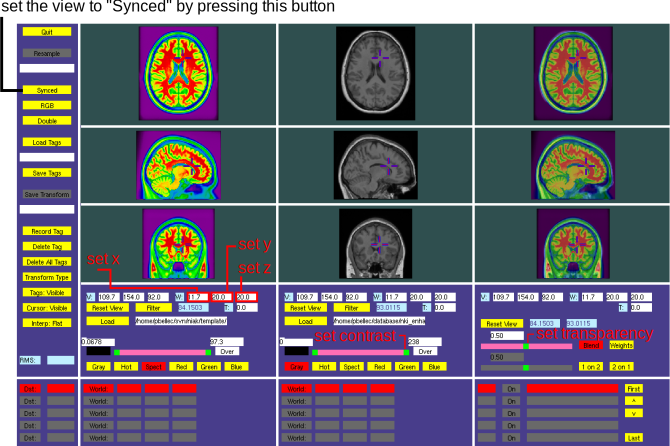
\includegraphics[width=\linewidth]{fig_set_slices}
\caption{The \texttt{register} interface}
\label{fig_set_slices}
\end{center}

\end{figure}

\subsection{Starting the raw datasets QC}

First open a terminal, then change the directory to the raw data folder. Choose any subject's folder then start the QC  by displaying the anatomical and the functional image in \texttt{register}:

\begin{lstlisting}
cd /raw_data/subject_x
register functional_image.mnc.gz anatomical_image.mnc.gz
\end{lstlisting}

There is no gold standard on raw data QC. We elaborated some validation criterion based on our laboratory internal expertise for cases that should be flagged as "Maybe", "Fail" or "Ok". The "fail" cases my cause our preprocessing pipeline to fail. \\
Following are the criterion one should go over to ensure good quality of raw data:
\begin{enumerate}
\item Check that the center of the field of view of the BOLD ant T$_1$ image lies near to the center of the brain (See figure \ref{fig_qc_raw_data_ok} left and middle column). to-do so, set the  X Y Z coordinate to 0, then verify if the cross is well positioned at the center of the brain. A failed case is shown on figure \ref{fig_qc_raw_data_center_fail}
\item Check that the raw T$_1$ and BOLD images are roughly coregistered (See figure \ref{fig_qc_raw_data_ok} right column). A failed case is shown on figure \ref{fig_qc_raw_data_coregist_fail}
\end{enumerate}


\subsection{Coregistration of T$_1$ and T$_2$ image in the native space}

\subsubsection{Visual inspection}
\begin{table}[htbp]
\centering
\captionsetup{justification=centering,margin=2cm}
 \begin{tabular}{c|rrr}
 & $x$ (sagital) & $y$ (coronal) & $z$ (axial)\\
  \hline
 \textbf{View 1} & 0 & 0 & 0\\
 \end{tabular} 
 \caption{Coordinates for visual review of the coregistration between the T$_1$ and T$_2$ image in the native space.}
 \label{tab_coord_t1_raw}
\end{table}
 
 
\begin{figure}[htbp]
\begin{center}
\captionsetup{justification=centering,margin=2cm}
\includegraphics[width=1\linewidth]{fig_qc_raw_data_ok}
\caption{
{\textbf{Quality control of raw datasets -- View} ($0$,$0$,$0$).} {A successful case of well centered brain origin. (Source: ABIDE sample)}}
\label{fig_qc_raw_data_ok}
\end{center}
\end{figure}

\newpage
\subsubsection{Examples of failed brain center and possible fixes}

\begin{figure}[htbp]
\captionsetup{justification=centering,margin=2cm}
\begin{center}
\includegraphics[width=1\linewidth]{fig_qc_raw_data_center_fail}
\caption{
{\textbf{Quality control of raw datasets -- View} ($0$,$0$,$0$).} {A Failed case brain center origin. (Source: ABIDE sample)}
}
\label{fig_qc_raw_data_center_fail}
\end{center}
\end{figure}

\subsection*{How to correct it ?}
look at the step and the start of each axis with the following command \lstinline|mincinfo mprage.mnc|. The output would be something like this: 

\lstset{language=bash}
\begin{lstlisting}
dimension name         length         step        start
  --------------         ------         ----        -----
  zspace                    192      1.19792         -147
  yspace                    192      1.19792      -60.732
  xspace                    144         -1.2           85
\end{lstlisting}

If step is positive or negative change the start by adding the \lstinline| newStart=(Current Start Value In Mincinfo) - value in world coord|. following is an example of possible fix for this case:\\%
\\
\lstset{language=bash}
\begin{lstlisting}
minc_modify_header -dinsert xspace:start=-120 mprage.mnc
minc_modify_header -dinsert yspace:start=-120 mprage.mnc
minc_modify_header -dinsert zspace:start=-120 mprage.mnc
\end{lstlisting}

\subsubsection{Examples of failed coregistration of T$_1$ and T$_2$ image in the native space and possible fixe}
\begin{figure}[htbp]
\captionsetup{justification=centering,margin=2cm}
\begin{center}

\includegraphics[width=0.333\linewidth]{fig_qc_raw_data_coregist_fail}
\caption{
{\textbf{Quality control of raw datasets -- View} ($0$,$0$,$0$).} {A Failed case of raw data coregistration. (Source: ABIDE sample)}
}
\label{fig_qc_raw_data_coregist_fail}
\end{center}
\end{figure}
\subsection*{How to correct it ?}
In preprocesing script, set the T1-T2 coregistration option to 'center' like this: \lstinline|opt.anat2func.init= 'center'|. The 'center' option usually does more harm than good, but in a case you have a very big misalignment between the two images (say, 2 cm) it is worth to use it.

\newpage
\section{Quality control of preprocessed datasets}

\subsection{Starting the QC script}

First open a terminal, start octave with NIAK loaded in the search path. Then change the directory to the output folder of the fMRI preprocessing pipeline and start the QC script:

\begin{lstlisting}
cd /data/output_folder_fmri_preprocess
niak_qc_fmri_preproc
\end{lstlisting}

The script will automatically open the program \texttt{register} (Figure \ref{fig_set_slices}) with a number of images for visual examination. The program will also prompt you to enter the results of the quality control, as well as optional comments. Those will be saved in a spreadsheet file (comma-separated values, .csv) in the output folder of the preprocessing, called \texttt{qc\_report.csv}. To start the procedure again, simply delete this file.

Figure \ref{fig_set_slices} shows the \texttt{register} window, as called by the script. It represents the individual T$_1$ volume of one subject in stereotaxic non-linear space, along with the template used as target for coregistration. The figure oulines important controls to select the views, set the contrast and transparency of the fusion between the two images. We recommend to navigate the images at four selected views, each corresponding to coordinates in stereotaxic space, as listed in Table \ref{tab_coord_t1}. Figure \ref{fig_qc_anat} oultines which structures need to be visually checked for each view. The case presented in the figure is a successful case, where all structures have been corrrectly aligned. This case should be reported as ``\texttt{OK}'' on the command line.




\subsection{Coregistration between the T$_1$ image and stereotaxic space}

\subsubsection{Visual inspection}
\begin{table}[htbp]
\centering
\captionsetup{justification=centering,margin=2cm}
 \begin{tabular}{c|rrr}
 & $x$ (sagital) & $y$ (coronal) & $z$ (axial)\\
  \hline
 \textbf{View 1} & -8 & -20 & 60\\
 \textbf{View 2} & 15 & -20 & 20\\
 \textbf{View 3} & 30 & -25 & -15\\
 \textbf{View 4} & -30 & -25 & -15\\
 \end{tabular} 
 \caption{List of coordinates for visual review of the coregistration between the T$_1$ image and stereotaxic space.}
 \label{tab_coord_t1}
\end{table}


\begin{figure}[htbp]
\begin{center}
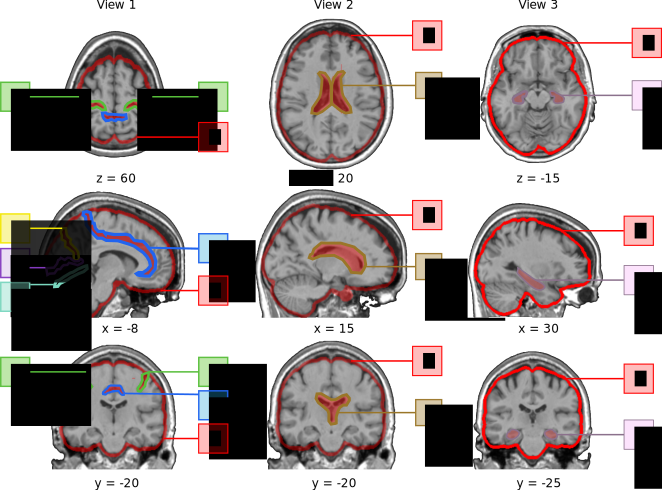
\includegraphics[width=\linewidth]{fig_qc_t1}
\end{center}
\caption{
{\textbf{Quality control of the structural coregistration}} {The anatomical landmarks that should be well aligned in a successful coregistration include: central sulcus (\textbf{A}), cingulate sulcus (\textbf{B}), parieto-occipital fissure (\textbf{C}), calcarine fissure (\textbf{D}), tentorium cerebellum (\textbf{E}), the lateral ventricles (\textbf{F}), the outline of the brain (\textbf{G}) and the hippocampal formation (\textbf{H}) bilateraly. The landmarks are outlined on an individual brain after successful non-linear coregistration in stereotaxic space.}
}
\label{fig_qc_anat}
\end{figure}

\newpage
\subsubsection{Examples of failed coregistration and possible fixes}
\label{sec-1}
\begin{figure}[h!tbp]
\begin{center}

\includegraphics[width=0.4\linewidth]{fig_qc_fail}
\end{center}
\caption{
{ Examples of failed coregistration between the T$_1$ volume and template space.} {The reference space for the panels is the template space (left image), and the correspondence between spaces is indicated with a cross located at identical coordinates in all three volumes. Note that this type of failures is generally due to problems with the origin of raw datasets. Sometimes hyperintensities in the structural image or large amount of fat tissues in the shoulder/neck areas can also cause failures.}
}
\label{fig_qc_fail}
\end{figure}

\subsection*{How to correct it ?}
 Check that the raw images are correct using the first section of this document. It is also possible to remove the shoulder/neck by cropping the image with minc command line, as follow:
\begin{lstlisting}
 mincreshape -clobber -dimrange zspace=60,180 <rawT1_image>.mnc.gz  <T1_image_cropped>.mnc.gz
\end{lstlisting}
 Here, it was determined by visual inspection using register that the brain began at z = 60 (voxel space) and ended around z = 240 (voxel space). So it was decided to set the start at 60 and then add a count of 180 (180 +60 = 240). The next section suggests another type of possible fix.

\subsubsection{Examples of a ``maybe'' coregistration and possible fixes}
\begin{figure}[h!tbp]
\begin{center}
\includegraphics[width=0.4 \linewidth]{fig_improve_qc}
\end{center}
\caption{
{The initial coregistration of an individual MRI with the target default NIAK template space (left image) failed locally, as the meninges around the brain were pushed inside the brain (middle image). This problem was related to a poor correction of non-uniformities in the image}
}
\label{fig_improve_qc}
\end{figure}
\subsection*{How to correct it ?}
A simple change of the parameter of the non-uniformity correction resulted in a successful coregistration (right image)

\lstset{language=matlab}
\begin{lstlisting}
opt.t1_preprocess.nu_correct.arg = '-distance 70'; % Parameter for non-uniformity correction . 200 is a suggested value for 1.5T images, 50 for 3T images. If you find that this stage did not work well, this parameter is usually critical to improve the results.
\end{lstlisting}
\newpage
\subsubsection{Example of ``grey area case'' with localized failure and correction}
\begin{figure}[htbp]
\begin{center}
\includegraphics[width=0.7\linewidth]{fig_qc_grey_case}

\end{center}
\caption{
{\bf Example of a ``grey area case'' with localized failure.} {The initial coregistration used as a target the default NIAK template space, i.e. the ICBM152 MNI non-linear (young healthy adult template), presented in the first row. The result of the coregistration is presented in the second row, where part of the meninges have been mistakenly coregistered with the brain, as indicated with a cross. The coregistration was improved by changing the parameter of non-uniformity correction.}
}
\label{fig_qc_grey_case}
\end{figure}

\subsection{Coregistration between the T$_1$ image and the mean BOLD volume}

\begin{table}[htbp]
\centering
\captionsetup{justification=centering,margin=2cm}
\label{tab_coord_bold}
 \begin{tabular}{c|rrr}
  & $x$ (sagital) & $y$ (coronal) & $z$ (axial)\\
  \hline
  \textbf{View 1} & 0 & -20 & 60\\
  \textbf{View 2} & 10 & -20 & 45\\
  \textbf{View 3} & 30 & -25 & -15\\
  \textbf{View 4} & -30 & -25 & -15\\
 \end{tabular} 
 \caption{List of coordinates for visual review of the coregistration between the T$_1$ image and mean BOLD volume.}
\end{table}


\begin{figure}[htbp]
\begin{center}
\includegraphics[width=\linewidth]{fig_qc_func}
\end{center}
\caption{
{\textbf{Quality control of the functional coregistration}} {The anatomical landmarks that should be well aligned in a successful coregistration include: central sulcus (\textbf{A}), cingulate sulcus (\textbf{B}), parieto-occipital fissure (\textbf{C}), calcarine fissure (\textbf{D}), tentorium cerebellum (\textbf{E}), the lateral ventricles (\textbf{F}), the hippocampal formation (\textbf{H}) and the outline of the brain (\textbf{G}) bilateraly. The landmarks are outlined on an individual brain after successful non-linear coregistration in stereotaxic space.}
}
\label{fig_qc_func}
\end{figure}


%\begin{figure}[htbp]
%\begin{center}
%\includegraphics[width=\linewidth]{fig_qc_func_ok}
%\end{center}
%\caption{
%{ Quality control of the coregistration between the T$_1$ volume and the mean BOLD volume.} {A successful case of coregistration between modalities. Examples of the major anatomical landmarks that will be checked on every individual brain to ensure the quality of the coregistration: parieto-occipital fissure and tentorium cerebellum (\textbf{a}), anterior and posterior cingulate sulcus (\textbf{b}), posterior cingulate sulcus (\textbf{c}), central and post-central sulci (\textbf{d}). For each slice, a zoom on the structure of interest is displayed (structure outlined in blue) for the mean functional (BOLD) volume and the T$_1$ scan of a signle individual from the ADNI2 sample.}
%}
%\label{fig_qc_func_ok}
%\end{figure}
\newpage
\subsection{Examples of failed coregistration T$_1$ and the BOLD image}
\begin{figure}[htbp]
\begin{center}
\includegraphics[width=0.4\linewidth]{fig_qc_fail_func}
\end{center}
\caption{
{ Example of failed coregistration T$_1$ and the BOLD image.}
}
\label{fig_qc_fail_func}
\end{figure}
\subsection*{How to correct it ?}
Same correction used in section \ref{sec-1} ,by cropping image.


\subsection{Examples of failed the BOLD image}
\begin{figure}[htbp]
\begin{center}
\includegraphics[width=0.8\linewidth]{fig_qc_fail_func2}
\end{center}
\caption{
{ Example of failed BOLD image due to wrong field of view positioning.}
}
\label{fig_qc_fail_func2}
\end{figure}
\subsection*{How to correct it ?}
Re-scan the participant or exclude the participant from the analysis. The field-of-view was not specified correctly during the acquisition.
\end{document}